\documentclass[12pt,twoside]{article}



%%%%%%%%%%%%%%%%%%%%%%%%%%%%%%%%%%%%%%%%%%%%%%%%%%%%%%%%%%%%%%%%%%%%%%%%%%%%%

% Definitions for the title page
% Edit these to provide the correct information
% e.g. \newcommand{\reportauthor}{Timothy Kimber}

\newcommand{\reporttitle}{An intelligent digital interface for sharing diagnostic medical imaging with patients}
\newcommand{\reportauthor}{Laura Hagege}
\newcommand{\supervisor}{Fernando Bello}
\newcommand{\degreetype}{Msc. Computing Science}

%%%%%%%%%%%%%%%%%%%%%%%%%%%%%%%%%%%%%%%%%%%%%%%%%%%%%%%%%%%%%%%%%%%%%%%%%%%%%

% load some definitions and default packages
%%%%%%%%%%%%%%%%%%%%%%%%%%%%%%%%%%%%%%%%%
% University Assignment Title Page 
% LaTeX Template
% Version 1.0 (27/12/12)
%
% This template has been downloaded from:
% http://www.LaTeXTemplates.com
%
% Original author:
% WikiBooks (http://en.wikibooks.org/wiki/LaTeX/Title_Creation)
%
% License:
% CC BY-NC-SA 3.0 (http://creativecommons.org/licenses/by-nc-sa/3.0/)
% 
%
%%%%%%%%%%%%%%%%%%%%%%%%%%%%%%%%%%%%%%%%%
%----------------------------------------------------------------------------------------
%	PACKAGES AND OTHER DOCUMENT CONFIGURATIONS
%----------------------------------------------------------------------------------------
\usepackage[a4paper,hmargin=2.8cm,vmargin=2.0cm,includeheadfoot]{geometry}
\usepackage{textpos}
\usepackage{natbib} % for bibliography
\usepackage{tabularx,longtable,multirow,subfigure,caption}%hangcaption
\usepackage{fncylab} %formatting of labels
\usepackage{fancyhdr} % page layout
\usepackage{url} % URLs
\usepackage[english]{babel}
\usepackage{amsmath}
\usepackage{graphicx}
\usepackage{dsfont}
\usepackage{epstopdf} % automatically replace .eps with .pdf in graphics
\usepackage{backref} % needed for citations
\usepackage{array}
\usepackage{latexsym}
\usepackage[pdftex,pagebackref,hypertexnames=false,colorlinks]{hyperref} % provide links in pdf

\hypersetup{pdftitle={},
  pdfsubject={}, 
  pdfauthor={},
  pdfkeywords={}, 
  pdfstartview=FitH,
  pdfpagemode={UseOutlines},% None, FullScreen, UseOutlines
  bookmarksnumbered=true, bookmarksopen=true, colorlinks,
    citecolor=black,%
    filecolor=black,%
    linkcolor=black,%
    urlcolor=black}

\usepackage[all]{hypcap}


%\usepackage{color}
%\usepackage[tight,ugly]{units}
%\usepackage{float}
%\usepackage{tcolorbox}
%\usepackage[colorinlistoftodos]{todonotes}
% \usepackage{ntheorem}
% \theoremstyle{break}
% \newtheorem{lemma}{Lemma}
% \newtheorem{theorem}{Theorem}
% \newtheorem{remark}{Remark}
% \newtheorem{definition}{Definition}
% \newtheorem{proof}{Proof}


%%% Default fonts
\renewcommand*{\rmdefault}{bch}
\renewcommand*{\ttdefault}{cmtt}



%%% Default settings (page layout)
\setlength{\parindent}{0em}  % indentation of paragraph

\setlength{\headheight}{14.5pt}
\pagestyle{fancy}
\renewcommand{\chaptermark}[1]{\markboth{\chaptername\ \thechapter.\ #1}{}} 

\fancyfoot[ER,OL]{\sffamily\textbf{\thepage}}%Page no. in the left on odd pages and on right on even pages
\fancyfoot[OC,EC]{\sffamily }
\renewcommand{\headrulewidth}{0.1pt}
\renewcommand{\footrulewidth}{0.1pt}
\captionsetup{margin=10pt,font=small,labelfont=bf}


%--- chapter heading

\def\@makechapterhead#1{%
  \vspace*{10\p@}%
  {\parindent \z@ \raggedright \sffamily
    \interlinepenalty\@M
    \Huge\bfseries \thechapter \space\space #1\par\nobreak
    \vskip 30\p@
  }}

%---chapter heading for \chapter*  
\def\@makeschapterhead#1{%
  \vspace*{10\p@}%
  {\parindent \z@ \raggedright
    \sffamily
    \interlinepenalty\@M
    \Huge \bfseries  #1\par\nobreak
    \vskip 30\p@
  }}

\allowdisplaybreaks

% load some macros
% Here, you can define your own macros. Some examples are given below.

\newcommand{\R}[0]{\mathds{R}} % real numbers
\newcommand{\Z}[0]{\mathds{Z}} % integers
\newcommand{\N}[0]{\mathds{N}} % natural numbers
\newcommand{\C}[0]{\mathds{C}} % complex numbers
\renewcommand{\vec}[1]{{\boldsymbol{{#1}}}} % vector
\newcommand{\mat}[1]{{\boldsymbol{{#1}}}} % matrix


\date{Juin 2018}

\begin{document}

% load title page
% Last modification: 2015-08-17 (Marc Deisenroth)
\begin{titlepage}

\newcommand{\HRule}{\rule{\linewidth}{0.5mm}} % Defines a new command for the horizontal lines, change thickness here


%----------------------------------------------------------------------------------------
%	LOGO SECTION
%----------------------------------------------------------------------------------------


\includegraphics[width = 4cm]{./figures/imperial}\\[0.5cm] 

\center % Center remainder of the page

%----------------------------------------------------------------------------------------
%	HEADING SECTIONS
%----------------------------------------------------------------------------------------

\textsc{\Large Imperial College London}\\[0.5cm] 
\textsc{\large Department of Computing}\\[0.5cm] 

%----------------------------------------------------------------------------------------
%	TITLE SECTION
%----------------------------------------------------------------------------------------

\HRule \\[0.4cm]
{ \huge \bfseries \reporttitle}\\ % Title of your document
\HRule \\[1.0cm]

%----------------------------------------------------------------------------------------
%	SUB TITLE SECTION
%----------------------------------------------------------------------------------------

\textsc{\large --- Background and Progress Report ---}\\[0.5cm] 
 
%----------------------------------------------------------------------------------------
%	AUTHOR SECTION
%----------------------------------------------------------------------------------------



\emph{by} \\
\reportauthor % Your name

~

\emph{Supervisor:} 
\supervisor % Supervisor's Name




%----------------------------------------------------------------------------------------
%	FOOTER & DATE SECTION
%----------------------------------------------------------------------------------------
\vfill % Fill the rest of the page with whitespace
Submitted in partial fulfillment of the requirements for the MSc degree in
\degreetype~of Imperial College London\\[0.5cm]

\makeatletter
\@date 
\makeatother


\end{titlepage}



% page numbering etc.
%\pagenumbering{roman}
%\clearpage{\pagestyle{empty}\cleardoublepage}
%\setcounter{page}{1}
%\pagestyle{fancy}

%%%%%%%%%%%%%%%%%%%%%%%%%%%%%%%%%%%%
%\begin{abstract}
%Your abstract.
%\end{abstract}

%\cleardoublepage
%%%%%%%%%%%%%%%%%%%%%%%%%%%%%%%%%%%%
%\section*{Acknowledgments}
%Comment this out if not needed.

\clearpage{\pagestyle{empty}\cleardoublepage}

%%%%%%%%%%%%%%%%%%%%%%%%%%%%%%%%%%%%
%--- table of contents
%\fancyhead[RE,LO]{\sffamily {Table of Contents}}
\tableofcontents 


\clearpage{\pagestyle{empty}\cleardoublepage}
\pagenumbering{arabic}
\setcounter{page}{1}
\fancyhead[LE,RO]{\slshape \rightmark}
\fancyhead[LO,RE]{\slshape \leftmark}

%%%%%%%%%%%%%%%%%%%%%%%%%%%%%%%%%%%%
\section{Project Overview}

\subsection{Supervisors}

My direct supervisor is Dr Fernando Bello, he is a computer scientist and engineer working at the intersection of medicine, education and technology. He is a Reader in Surgical Computing and Simulation Science at Imperial College London, where he co-directs the Centre for Engagement and Simulation Science, leading a multi-disciplinary research group aiming at building suitable models and simulations of clinical processes, including clinical examination, clinical diagnosis, interventional procedures and care pathways.
Dr Bello proposed my project as entitled "An intelligent digital interface for sharing diagnostic medical imaging with patients".\\

I am also working with William Cox, which is currently working on a PhD project investigating the extraction of novel benefit from diagnostic radiological images through sharing images with patients.\\ 

Dr Bello and Mr Cox will be together supporting my project and providing me informations, feed-back and support for its realization. \\


\subsection{Project Goal}


The aim of this project is to create a graphical user interface (GUI) that allows MRI, CT-scan, X-Ray patients to access their datas, with different levels of “benefits”. Data acquisition through this interface should be valuable for patients. \\
Following the first meeting with my tutors I have been able to define main criteria of success concerning the creation of the interface:
\begin{itemize}
\item Patient should be able to understand provided images 
\item Patient could explore the data in different ways/ different images orientation
\item Patient should have the possibility to ask questions to doctors/ specific assigned people
\end{itemize}
I have used those basis criteria to create further specifications to meet my supervisors needs.\\

Some tools are already existing but essentially for dorctors; my tutors are expecting me to create something similar to the existing available interfaces but in a version that is understandable/usable for a non clinical person. The idea is to look at existing interface designs and consider how they could be changed in order to make them user friendly for the specified user group more accessible/intuitive.


\end{itemize}



\clearpage
%%%%%%%%%%%%%%%%%%%%%%%%%%%%%%%%%%%%
\section{Background Work}


\subsection{Project field apprehension:} 
Towards the first meeting with my supervisors, Will have emailed me several documents in order to get myself familiar with the context of which my project is part of.
Those documents included:
\begin{itemize}
\item William PhD late stage review report discussing the benefit of creating a patient oriented interface
\item A Litterature review document called "Patient Health Record Systems Scope and Functionalities" [4]
\item A Litterature review document called "Patient Portal Preferences: Perspectives on Imaging Information" [5]
\item A research article entitled "Imaging informatics for consumer health: towards a radiology patient portal"
\end{itemize}
 
\subsection{Project frame and specifications definition:}
Before starting coding the interface, it is important to define the specifications in the most precise way with my tutors in order to be sure that the future produced work will fit their needs. \\
Specification should be done considering:
\begin{itemize}
\item Interface oriented specification:
\begin{itemize}
\item Content
\item Functionalities
\item Design
\end{itemize}

\item Data Providing:
\begin{itemize} 
\item What can be provided?
\item How to provide it?
\end{itemize}

	
\end{itemize}

\clearpage

\subsection{DICOM Data familiarization}
Imaging datas are provided in a specific format called DICOM - Digital Imaging and Communication in Medicine. This is a standard format for storing and transmitting informatic data related to medical images. This has been widely adpoted by most hospitals in order to standardise data transmission between different radiology tools – such as scanners servers, workstation, printers, network hardware and PACS - Picture Archiving and Communication System – and different stakeholders.  \\
DICOM data readers exist in open-source over the internet, my first work conerning those data is to explore existing readers and pick one that could suits my project.
 

\subsection{Choose accurate implementation method:}
I have been given the freedom to choose the langage and tools that I will use to create the interface. Multiple GUI tools are provided on the Internet, along with tutorials and advices to create interfaces. Before starting to implement the interface it is important to choose the tool that will best fit my needs. Exploring the Internet, the idea is to make a short comparison between the current most famous tools and choose the one that I feel the most confortable with.




\clearpage
%%%%%%%%%%%%%%%%%%%%%%%%%%%%%%%%%%%%
\section{LSEPI Checklist}

\begin{figure}[ht]
\centering
\includegraphics[width = 0.99\hsize]{./figures/LSEPI-CL1}
\caption{LSEPI Checklist - part 1}
\end{figure}

\clearpage

\begin{figure}[tb]
\centering
\includegraphics[width = 0.99\hsize]{./figures/LSEPI-CL2}
\caption{LSEPI Checklist - part 2}
\end{figure}


\clearpage
%%%%%%%%%%%%%%%%%%%%%%%%%%%%%%%%%%%%
\section{Progress Sumarry}

From now a large amount of work has been completed concerning the background and I'll be soon begin to develop a first prototype of the interface. Current achieved steps are defined below.

\subsection{Project field apprehension}
Before the first meeting with my tutors I have read the given documents in order to get familiar with the future project. I have also made some research appart relating relevant vocabulary and informations.
Moreover, reading William PhD's report which measure the benefit of creating such a patient oriented interface I realized how profitable my future work could be to imaging patient.


\subsection{Specification Definition}
We have had several discussions with my tutors concerning their expectation according to the interface, following which we agreed on the project specifications - that might evolve during the realization of the interface.
\begin{itemize}
	
\item \textbf{Interface content:}
\begin{itemize}
\item The interface should display patient images - images will be provided in DICOM format, and translated so that the patient can read them.
\item The interface must contain the clinical report and the simplifie version.
\item A link to NHS website will be given, so that patient could find general informations about their condition
\item Patient could get flag informations - to be filled by doctors - while exploring the images
\item Any other relevant informations related to what the DICOM files provides could be added 
\end{itemize}

\item \textbf{Interface functionalities:} \\ \\
The interface should provide:
\begin{itemize}
\item One doctor oriented window: so, they can fill in datas (images, report) and add flag to images at their conveniance.
\item One patient oriented window: read only data (no modification allowed) and the possibility for patient to chat with doctors.

\end{itemize}

My main concern - in the context of this project - is to focus on the patient oriented side and see how far I can lead this project. This part can be really time consuming as it might need to be oftently readapted following the needs of my tutors.

Also, William recently sent me detailed general specifications concerning the patient oriented interface content/functions - Appendix 1


\item \textbf{Interface design:}
\begin{itemize}
\item Imaging display will depend on the provided images (MRI, CT) but not on the part of the body. Will also gave me on demand description concerning images to be display and the way to deal with it – Appendix 2.
\item Provide a side by side – or other relevant organization – that would allow the patient to get the images and the report together in a relevant way

\end{itemize}

\item \textbf{Further precisions:}
\begin{itemize}
\item No access to any database will be provided for the current project (security issues) 
\item Access to the interface will be local – patient would be given (upon request) a CD with their images loaded on the interface; this won’t change patient access to datas but should make them want to access it
\item Interface should include user specification/precisions for patient 
\item Benefits/specifications will have to be defined before starting implementation
\item Interface should be “windows portable” 
\end{itemize}

\item \textbf{Interface evaluation:} \\ \\
At some point the interface should be evaluted by a panel of patient that would be ask to use it and make feedbacks.


\end{itemize}

\clearpage


\subsection{GUI tool choice: Qt}
A lot of tools are available on the Internet to create GUI interface such as Qt, WxWidget, GTK+, FLTK, FOX and some others. I couldn't compare all of them so I have decided to focus on Qt, WxWidget GTK+.

\begin{itemize} 
\item Tools Comparison: \\
I looked accross the Internet to get some testimonies about the different tools and I tried to distinguish them following several criteria - see grid below. 
According to these criteria and considering that Qt is highly recommended for beginners, I have finally decided to use Qt for this project.

\begin{figure}[ht]
\centering
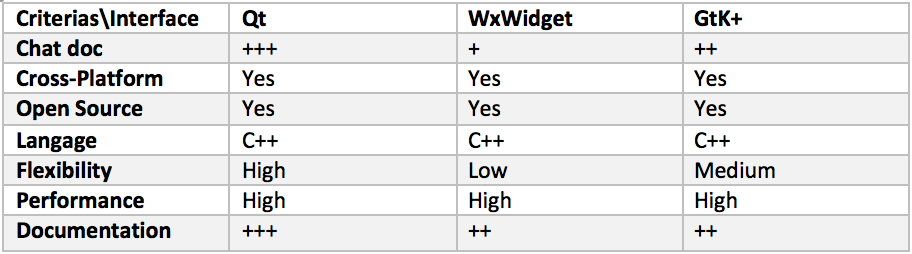
\includegraphics[width = 0.99\hsize]{./figures/comparison}
\caption{LQt, WxWidget, GTK+ comparison table}
\end{figure}
 
\item Qt familiarization: \\
In order to get used to this new tools I have decided to do Openclassroom tutorials [2].
Those tutorials have helped me to install QtCreator and to begin with some basic exercices to get familiar with Qt. I still have some tutorial to do at the current moment but I am feeling comfortable with it.
 
	
\end{itemize}

\subsection{DICOM apprehension}
DICOM files are containing a large amount of data and cannot be read so easily. Several readers are provided towards the internet. Currently I am planning to use QtDcm [1] that provide a reader suitable for Qt application, I have download the widget but the installation seems to be more complicated than I thought.


\clearpage
%%%%%%%%%%%%%%%%%%%%%%%%%%%%%%%%%%%%
\section{Project Plan}
From now I need in the short term to complete my backgound work which I expect to be done on the 15th June, consisting now in:

\begin{itemize} 
\item Getting familiar with DICOM readers and display DICOM images
\item Finish Qt tutorials
\item Create a grid concerning the informations to be display
\item Look on the web existing interface to get on a idea of what I could do
\item Make a design proposal
\end{itemize}	


I am then aiming to propose to my tutors a first draft of the interface by the end of this month (30th June). The following month will be to precise content, featuring and discuss rearrangement as the interface is evolving.
We agree with my tutors that the essential goal of my project will be to produce the patient oriented window because there is already a lot of work that can be done. If I have more time, I will use it to create the doctor oriented window.









\clearpage
%%%%%%%%%%%%%%%%%%%%%%%%%%%%%%%%%%%%
\section{Appendix}
\subsection {Appendix 1 - General Interface Specification}

\begin{figure}[ht]
\centering
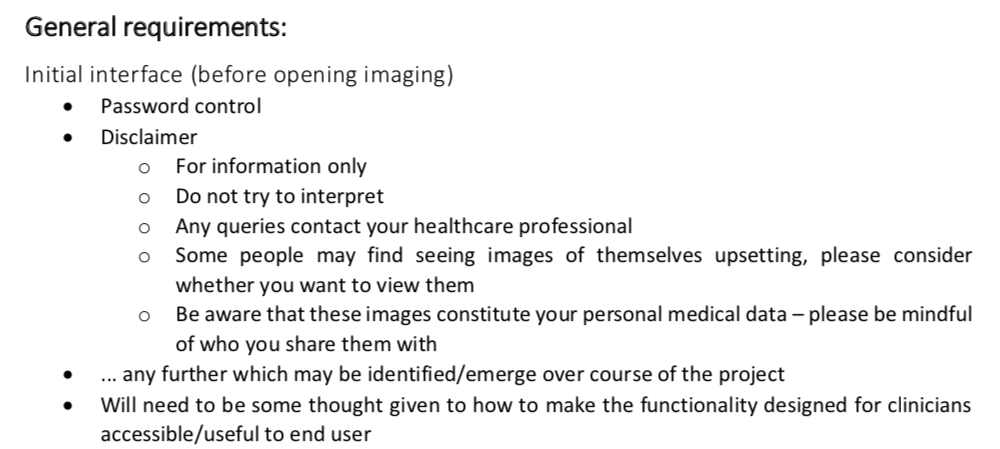
\includegraphics[width = 0.95\hsize]{./figures/GeneralSpec1}
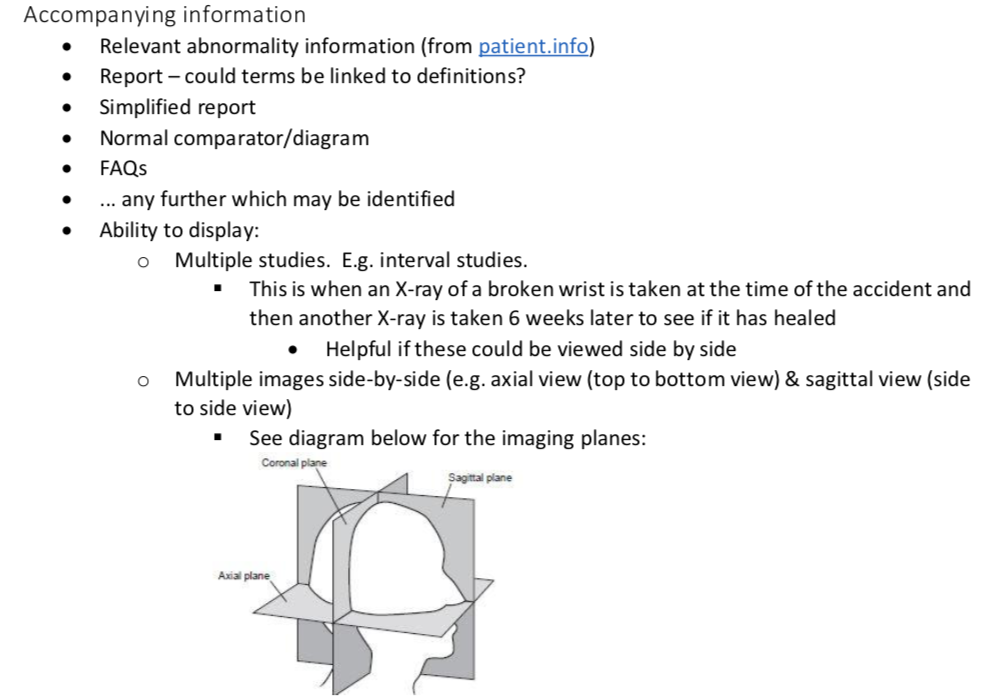
\includegraphics[width = 0.95\hsize]{./figures/GeneralSpec2}
\end{figure}



\clearpage

\begin{figure}[ht]
\centering
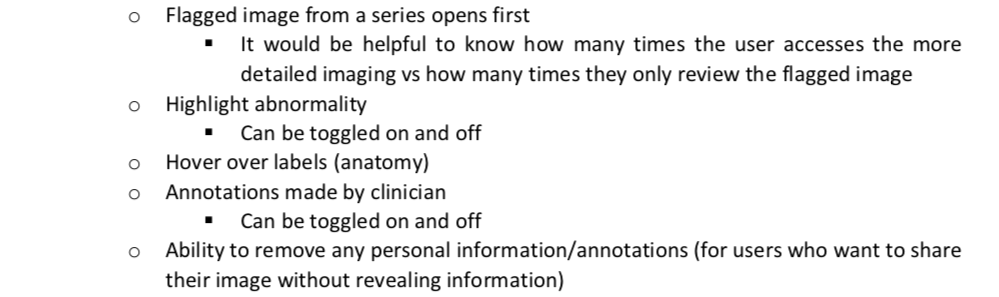
\includegraphics[width = 0.95\hsize]{./figures/GeneralSpec3}
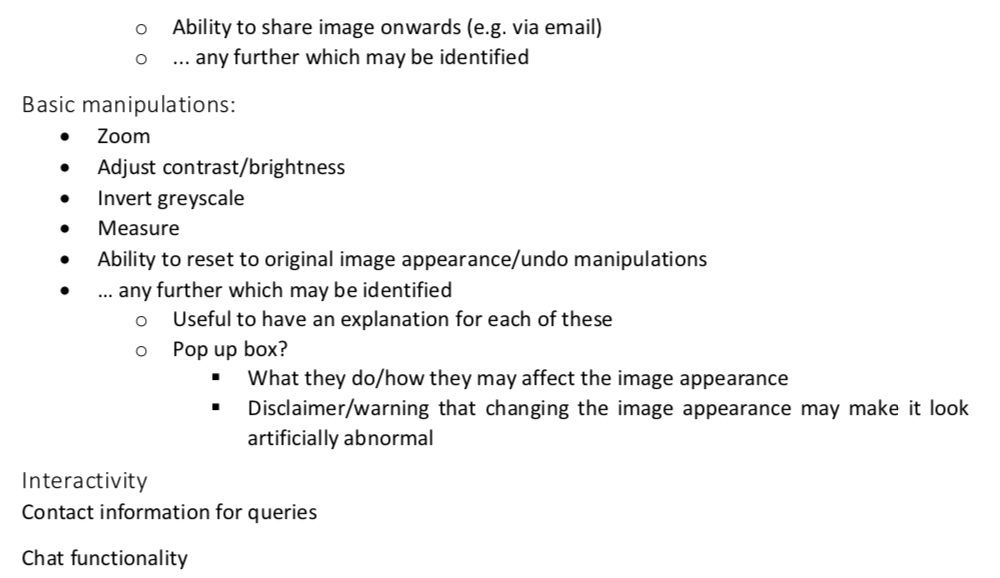
\includegraphics[width = 0.95\hsize]{./figures/GeneralSpec4}
\end{figure}

\clearpage

\subsection {Appendix 2 - Imaging Specification}

\begin{figure}[ht]
\centering
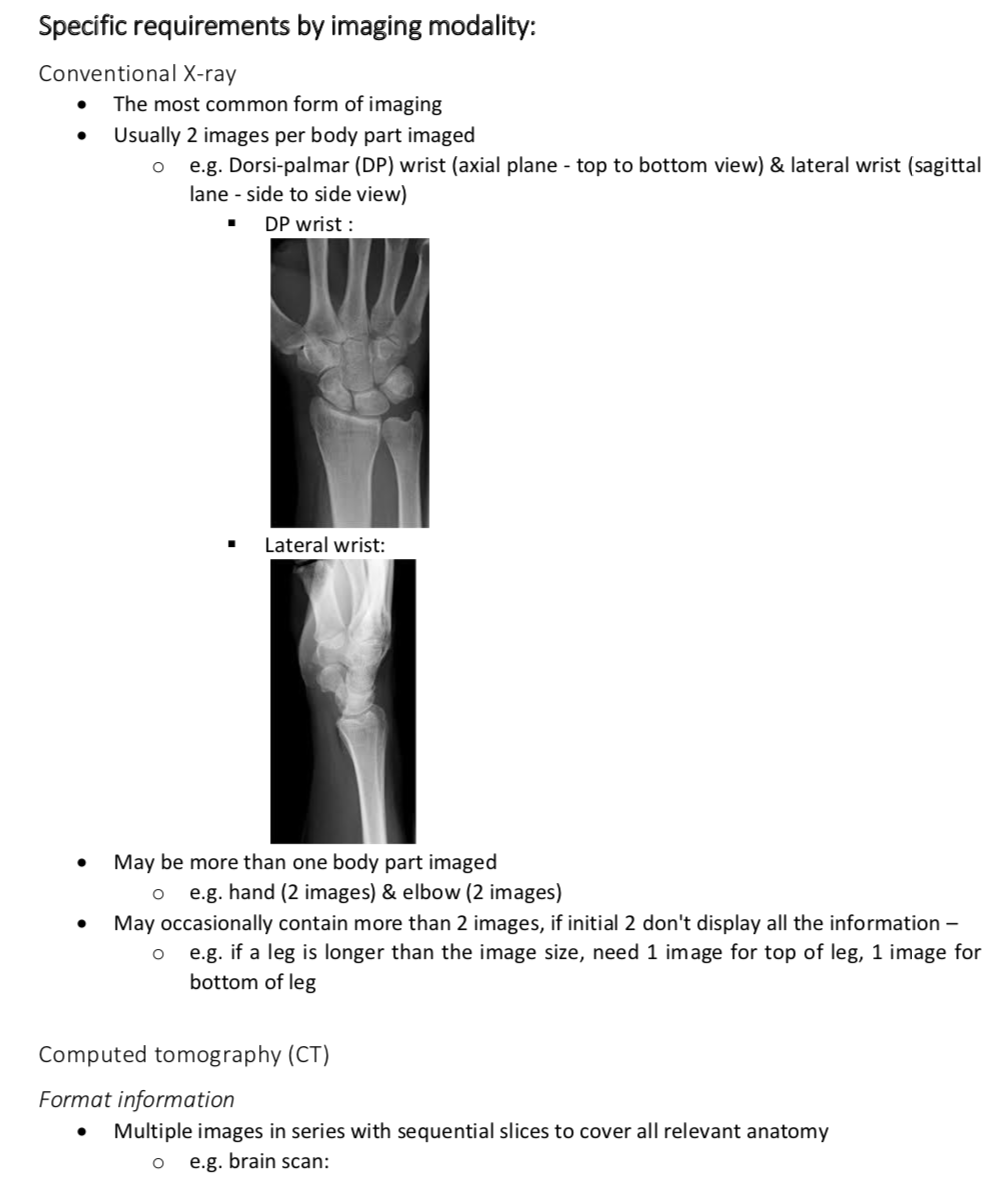
\includegraphics[width = 0.95\hsize]{./figures/ImagingSpec1}
\end{figure}
\clearpage

\begin{figure}[ht]
\centering
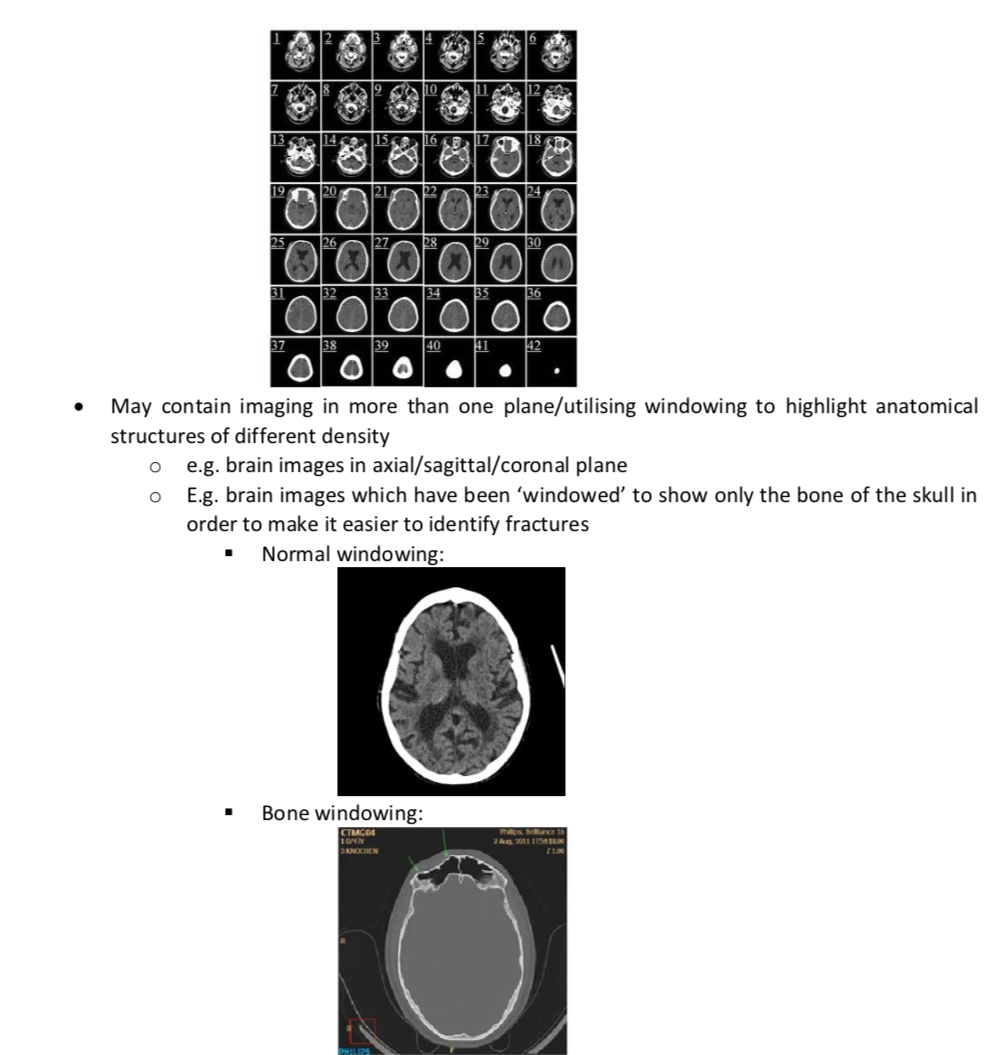
\includegraphics[width = 0.95\hsize]{./figures/ImagingSpec2}
\end{figure}
\clearpage

\begin{figure}[ht]
\centering
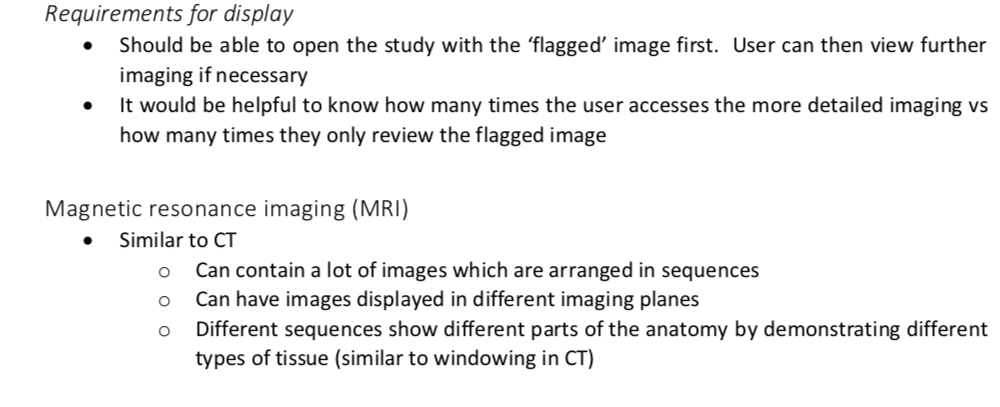
\includegraphics[width = 0.95\hsize]{./figures/ImagingSpec3}
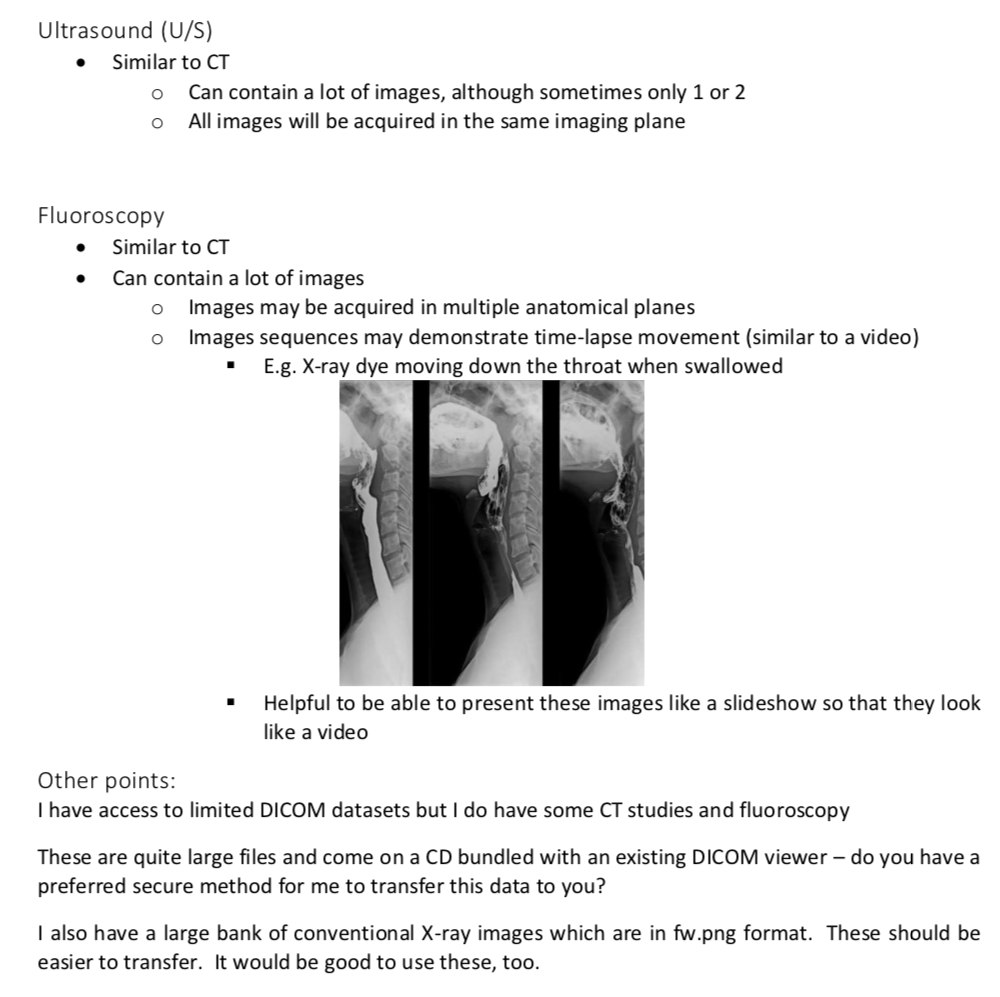
\includegraphics[width = 0.95\hsize]{./figures/ImagingSpec4}
\end{figure}
\clearpage



%% bibliography
\section{Bibliography}

\begin{figure}[ht]
\centering
\includegraphics[width = 0.99\hsize]{./figures/biblio}
\end{figure}
\clearpage




\end{document}
